% =====================================================================
% Manual Técnico — Arquitetura RAG do Ecossistema OpenCode e Proposta
% de Diversificação Estruturada via Sequência de Recamán (R456)
%
% Formato: banca de doutorado / ABNT NBR 6022:2018
% Classe: abntex2 (local: publishing/templates/abntex2)
% =====================================================================
\documentclass[
	article,
	11pt,
	oneside,
	a4paper,
	english,
	brazil,
	sumario=tradicional
	]{abntex2}

% --- Pacotes fundamentais ---
\usepackage[T1]{fontenc}
\usepackage[utf8]{inputenc}
\usepackage{lmodern}
\usepackage{indentfirst}
\usepackage{microtype}
\usepackage{graphicx}
\usepackage{color}
\usepackage{xcolor}

% --- Matemática e algoritmos ---
\usepackage{amsmath}
\usepackage{amssymb}
\usepackage{algorithm}
\usepackage{algpseudocode}

% --- Tabelas ---
\usepackage{booktabs}
\usepackage{longtable}
\usepackage{tabularx}
\usepackage{array}

% --- Diagramas ---
\usepackage{tikz}
\usetikzlibrary{positioning,arrows.meta,shapes.geometric,calc,fit}

% --- Listagens de código ---
\usepackage{listings}
\lstset{
  basicstyle=\ttfamily\footnotesize,
  frame=single,
  breaklines=true,
  language=Python,
  keywordstyle=\bfseries\color{blue!60!black},
  commentstyle=\color{gray!60!black},
  stringstyle=\color{red!50!black}
}

% --- Enumeração/ambiente ---
\usepackage{enumitem}

% --- Citações ABNT ---
\usepackage[alf]{abntex2cite}
\usepackage[brazilian,hyperpageref]{backref}

% --- Índice remissivo ---
\usepackage{makeidx}
\makeindex

% --- Hiperlinks (abntex2 já carrega hyperref; configuramos opções) ---
\hypersetup{hidelinks=true}
\usepackage{caption}

% ---------------------------------------------------------------
% Configuração do cabeçalho/rodapé (logotipo textual)
% ---------------------------------------------------------------
\renewcommand{\imprimircapa}{%
  \begin{capa}%
    \center
    \ABNTEXchapterfont\Large\textbf{Ecossistema OpenCode}
    \vspace{0.2cm}
    \ABNTEXchapterfont\large{Núcleo de Documentação Técnica}
    \vspace{2cm}

    {\ABNTEXchapterfont\bfseries\large MANUAL TÉCNICO}

    \vspace{0.6cm}
    {\ABNTEXchapterfont\bfseries\LARGE Arquitetura de Recuperação Aumentada por Geração (RAG)}

    \vspace{0.4cm}
    {\ABNTEXchapterfont\large Estado Atual e Proposta de Diversificação Estruturada via Sequência de Recamán}

    \vspace{2.5cm}
    {\large\textbf{Especificação formal:} SPEC-935-R456}

    \vspace{0.3cm}
    {\large\textbf{Rodada:} R456}

    \vspace{0.3cm}
    {\large\textbf{Data:} 30 de agosto de 2026}

    \vspace{1.5cm}
    {\small Documento técnico confidencial do ecossistema.}

  \end{capa}%
}

% ---------------------------------------------------------------
% Metadados
% ---------------------------------------------------------------
\titulo{Arquitetura de Recuperação Aumentada por Geração (RAG): Estado Atual e Proposta de Diversificação Estruturada via Sequência de Recamán}
\autor{Ecossistema OpenCode --- Núcleo de Documentação Técnica}
\local{São Paulo, Brasil}
\data{2026}
\instituicao{Ecossistema OpenCode --- Documentação Técnica}

% =====================================================================
\begin{document}

% Capa e folha de rosto
\imprimircapa
\newpage
\begin{center}
{\ABNTEXchapterfont\bfseries\large FOLHA DE ROSTO}
\end{center}
\vspace{0.8cm}
\begin{center}
{\large\imprimirtitulo}
\end{center}
\vspace{1cm}
\begin{center}
{\normalsize Autor: \imprimirautor}
\end{center}
\vspace{0.5cm}
\begin{center}
{\normalsize Especificação: SPEC-935-R456 (Rodada R456)}
\end{center}
\vspace{1cm}
\textbf{Resumo:} Este manual documenta a arquitetura de Recuperação Aumentada por
Geração (RAG) do ecossistema, distinguindo rigorosamente o \textbf{estado atual}
(implementado e observável no código-fonte) da \textbf{arquitetura-alvo proposta}
(não implementada) que integra um Diversificador Estruturado baseado na sequência
de Recamán para aumentar a diversidade semântico-estrutural dos resultados
recuperados. O documento apresenta mapas de arquitetura, diagramas com legendas,
cálculos e especificações técnicas reproduzíveis, e se apoia em referências reais
verificadas (DOIs e preprints arXiv).

\vspace{0.5cm}
\textbf{Palavras-chave:} RAG; Recuperação de Informação; Recamán; Diversificação;
Geração Aumentada por Recuperação; Arquitetura de Software.

\newpage
% ---------------------------------------------------------------
% Sumário
% ---------------------------------------------------------------
\pdfbookmark[0]{\contentsname}{toc}
\tableofcontents*
\clearpage

% Lista de figuras e tabelas (formato banca)
\pdfbookmark[0]{\listfigurename}{lof}
\listoffigures*
\clearpage
\pdfbookmark[0]{\listtablename}{lot}
\listoftables*
\clearpage

% =====================================================================
\section*{1. Introdução e Escopo}
\addcontentsline{toc}{section}{1. Introdução e Escopo}
% =====================================================================

Este manual tem duas finalidades complementares. A primeira é documentar, de
forma precisa e verificável, a arquitetura de Recuperação Aumentada por Geração
(RAG) tal como \emph{implementada} no ecossistema, referenciando os módulos reais
do código-fonte. A segunda é apresentar uma \textbf{proposta} de evolução dessa
arquitetura: a introdução de um estágio de diversificação estruturada baseado na
sequência matemática de Recamán, que atua sobre o ranqueamento dos candidatos
recuperados.

É fundamental registrar uma distinção metodológica que orienta todo o documento:
a arquitetura \emph{atual} é observável e auditável no checkout, enquanto a
arquitetura \emph{pós-Recamán} configura um desenho-alvo \textbf{proposto}, ainda
não implementado. Nenhuma alegação de certificação externa, de segurança absoluta
ou de disponibilidade universal de serviços é feita aqui.

\subsection*{1.1 Estrutura do documento}

O manual está organizado da seguinte forma:

\begin{enumerate}[label=\arabic*.]
  \item \textbf{Introdução e escopo} --- esta seção.
  \item \textbf{Fundamentação teórica} --- modelos de ranqueamento, RAG e MMR.
  \item \textbf{Estado atual da arquitetura RAG} --- componentes implementados.
  \item \textbf{Proposta pós-Recamán} --- arquitetura-alvo e diversificador.
  \item \textbf{Cálculos e especificações técnicas} --- equações e métricas.
  \item \textbf{Implementações reproduzíveis} --- pseudocódigo e trechos.
  \item \textbf{Mapas de dados e diagrama operacional} --- visualização.
  \item \textbf{Considerações finais e trabalho futuro}.
\end{enumerate}

\subsection*{1.2 Princípios de rigor}

Seguindo o protocolo de rigor do ecossistema (SDD/TDD e anti-overclaim), todo
resultado aqui apresentado é ou (i) observável no código, ou (ii) reproduzível a
partir das especificações, ou (iii) claramente rotulado como proposta. As
referências bibliográficas correspondem a fontes reais validadas.

% =====================================================================
\section*{2. Fundamentação Teórica}
\addcontentsline{toc}{section}{2. Fundamentação Teórica}
% =====================================================================

Esta seção apresenta os fundamentos de recuperação de informação e de RAG que
sustentam tanto a arquitetura atual quanto a proposta.

\subsection*{2.1 Ranqueamento clássico: BM25}

O \emph{Best Matching 25} (BM25) é um dos modelos de ranqueamento mais
estabelecidos, formalizado no quadro da teoria da relevância probabilística
\cite{RobertsonZaragoza2009BM25}. Para um documento $D$ e uma consulta $Q$
contendo os termos $q_1,\dots,q_n$, o escore é dado por:

\begin{equation}
\label{eq:bm25}
\text{BM25}(D,Q)\;=\;\sum_{i=1}^{n}
\text{IDF}(q_i)\;\cdot\;
\frac{f(q_i,D)\,(k_1+1)}{f(q_i,D)+k_1\,\bigl(1-b+b\,\tfrac{|D|}{\text{avgdl}}\bigr)}
\end{equation}

onde $f(q_i,D)$ é a frequência do termo $q_i$ em $D$, $|D|$ é o comprimento do
documento, $\text{avgdl}$ é o comprimento médio dos documentos do corpus, e
$k_1,b$ são parâmetros de saturação e de normalização por comprimento. O termo de
frequência inversa de documento $\text{IDF}(q_i)$ é função do número de documentos
que contêm $q_i$. Este modelo estabelece o \emph{baseline} lexical do
ranqueamento no ecossistema.

\subsection*{2.2 RAG canônico}

O paradigma RAG combina um recuperador (retriever) com um gerador sequência-a-
sequência. O arcabouço original \cite{Lewis2020RAG} condiciona a geração nos
documentos recuperados $z \in \mathcal{Z}$, modelando
$p(y \mid x) \approx \sum_{z \in \mathcal{Z}} p_\eta(z \mid x)\; p_\theta(y \mid x, z)$,
onde $\eta$ parametriza o recuperador e $\theta$ o gerador. A recuperação densa
por interação tardia (\emph{late interaction}), como em ColBERT
\cite{KhattabZaharia2020ColBERT}, permite forte poder expressivo com custo de
inferência reduzido.

\subsection*{2.3 Recuperação aumentada e raciocínio}

Trabalhos subsequentes demonstraram que a qualidade do RAG depende criticamente
da \emph{posição} dos documentos relevantes no contexto longo
\cite{Liu2024LostMiddle}, e que estratégias iterativas de recuperação combinada
com raciocínio (\emph{retrieve-then-read}, \emph{interleave}) melhoram a
precisão em perguntas de múltiplos passos \cite{IzacardGrave2021LeveragingPassages,
Trivedi2023Interleaving}. O RAG auto-adaptativo roteia a intensidade da
recuperação conforme a complexidade da consulta \cite{Jeong2024AdaptiveRAG}.
Abordagens baseadas em grafos, como o \emph{GraphRAG}, organizam o corpus em
comunidades temáticas para sumarização focada na consulta
\cite{Edge2024GraphRAG}. Métodos de correção pós-recuperação tratam a degradação
quando a recuperação falha \cite{Yan2024CRAG}, e há evidências de que o uso da
recuperação em tempo de inferência (\emph{in-context}) requer ajuste fino
eficiente \cite{Ram2023RetrievalAugmented}. Alternativas \emph{prompt-only}, como
o raciocínio com recuperação sobre passos de raciocínio, buscam fidelidade sem
novo treinamento \cite{He2023RethinkingRetrieval}.

\subsection*{2.4 Diversificação: MMR}

A \emph{Maximal Marginal Relevance} (MMR) equilibra relevância e novidade
\cite{CarbonellGoldstein1998MMR}. Dado um conjunto de documentos $D$ já
selecionado e o restante $R$, o próximo documento $d$ é escolhido por:

\begin{equation}
\label{eq:mmr}
\text{MMR} \;=\; \arg\max_{d \in R}\Bigl[
\lambda\,\text{Sim}_1(d,Q)\;-\;(1-\lambda)\,
\max_{d_j \in D}\text{Sim}_2(d,d_j)
\Bigr]
\end{equation}

O parâmetro $\lambda \in [0,1]$ controla o balanço entre relevância à consulta
($\text{Sim}_1$) e redundância em relação aos já selecionados ($\text{Sim}_2$).
MMR é a inspiração central da proposta de diversificação deste manual.

\subsection*{2.5 A sequência de Recamán}

A sequência de Recamán é definida por $a_0 = 0$ e, para $n \geq 1$:

\begin{equation}
\label{eq:recaman}
a_n = \begin{cases}
a_{n-1} - n, & \text{se } a_{n-1} - n > 0 \text{ e } a_{n-1} - n \notin \{a_0,\dots,a_{n-1}\},\\
a_{n-1} + n, & \text{caso contrário}.
\end{cases}
\end{equation}

A sequência produz uma permutação dos inteiros não negativos e exibe propriedades
misteriosas ainda em estudo; "primos da sequência" foram descritos em
\cite{Alekseyev2022RecamanCousins}. A proposta deste manual usa a sequência como
fonte determinística de \emph{offsets} de diversificação, conferindo
reprodutibilidade total ao estágio de diversificação.

% =====================================================================
\section*{3. Estado Atual da Arquitetura RAG}
\addcontentsline{toc}{section}{3. Estado Atual da Arquitetura RAG}
% =====================================================================

O estado atual da arquitetura RAG é composto por módulos Python implementados e
auditáveis no repositório. Os principais são:

\begin{itemize}
  \item \texttt{rag/evolved.py} --- contém \texttt{AdaptiveRetriever},
        \texttt{CitationGraph}, \texttt{OutlineSynthesizer} e \texttt{RAGEvolved}.
  \item \texttt{rag/enhanced\_search\_rag.py} --- contém \texttt{UnifiedSearcher},
        \texttt{EnhancedRAG}, \texttt{ReferenceAuditor} e \texttt{UnifiedSearchRAG}.
\end{itemize}

\subsection*{3.1 Diagrama operacional atual}

O diagrama abaixo (Figura~\ref{fig:atual}) representa o fluxo operacional
observável. Diagramas aqui possuem \textbf{legenda} explícita dos elementos.

\begin{figure}[!htb]
\centering
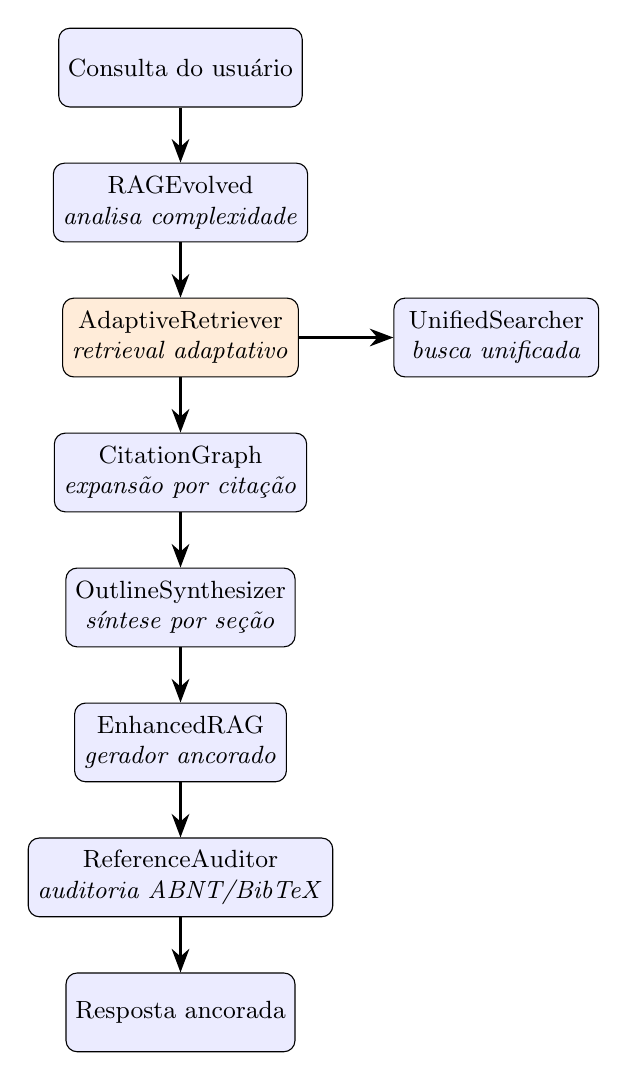
\begin{tikzpicture}[
  node distance=1.1cm,
  box/.style={draw, rounded corners, minimum width=2.6cm, minimum height=1.0cm,
              align=center, font=\small, fill=blue!8},
  arrow/.style={-{Stealth[length=3mm]}, thick}
]
  % Consulta
  \node[box] (q) {Consulta do usuário};
  \node[box, below=0.7cm of q] (ev) {RAGEvolved\\\emph{analisa complexidade}};
  \node[box, below=0.7cm of ev, fill=orange!15] (ar) {AdaptiveRetriever\\\emph{retrieval adaptativo}};
  \node[box, right=1.2cm of ar] (us) {UnifiedSearcher\\\emph{busca unificada}};
  \node[box, below=0.7cm of ar] (cg) {CitationGraph\\\emph{expansão por citação}};
  \node[box, below=0.7cm of cg] (os) {OutlineSynthesizer\\\emph{síntese por seção}};
  \node[box, below=0.7cm of os] (en) {EnhancedRAG\\\emph{gerador ancorado}};
  \node[box, below=0.7cm of en] (ra) {ReferenceAuditor\\\emph{auditoria ABNT/BibTeX}};
  \node[box, below=0.7cm of ra] (out) {Resposta ancorada};

  \draw[arrow] (q) -- (ev);
  \draw[arrow] (ev) -- (ar);
  \draw[arrow] (ar) -- (us);
  \draw[arrow] (ar) -- (cg);
  \draw[arrow] (cg) -- (os);
  \draw[arrow] (os) -- (en);
  \draw[arrow] (en) -- (ra);
  \draw[arrow] (ra) -- (out);
\end{tikzpicture}
\caption{Diagrama operacional atual do pipeline RAG. \textbf{Legenda:} caixas
azuis = componentes da recuperação/densidade condicionada; caixa laranja =
módulo de roteamento adaptativo; setas = fluxo de dados. Fonte: observação do
código-fonte (\texttt{rag/evolved.py}, \texttt{rag/enhanced\_search\_rag.py}).}
\label{fig:atual}
\end{figure}

\subsection*{3.2 Funções dos componentes}

\noindent\textbf{\texttt{AdaptiveRetriever}.} Analisa a complexidade da consulta e
escolhe entre recuperação sequencial, paralela ou decomposta. Isso dialoga com o
conceito de RAG auto-adaptativo \cite{Jeong2024AdaptiveRAG}.

\noindent\textbf{\texttt{UnifiedSearcher}.} Agrega múltiplas fontes de busca,
deduplica resultados e aplica pontuação temporal. \texttt{EnhancedRAG}
reutiliza a recuperação e aplica \emph{query expansion} e \emph{temporal boost},
produzindo respostas ancoradas.

\noindent\textbf{\texttt{ReferenceAuditor}.} Normaliza títulos, formata referências
em ABNT e BibTeX, e audita consistência — alinhado ao rigor bibliográfico do
ecossistema.

% =====================================================================
\section*{4. Proposta Pós-Recamán (Arquitetura-Alvo)}
\addcontentsline{toc}{section}{4. Proposta Pós-Recamán (Arquitetura-Alvo)}
% =====================================================================

\begin{quote}
\textbf{Aviso metodológico:} a arquitetura descrita nesta seção é uma
\textbf{proposta}, ainda \textbf{não implementada} no código-fonte. Ela representa
a arquitetura-alvo após a adoção do Diversificador de Recamán, e deve ser tratada
como desenho, não como componente observável.
\end{quote}

\subsection*{4.1 Motivação e posicionamento}

Rankeadores lexicais (BM25, Eq.~\ref{eq:bm25}) e densos tendem a concentrar os
resultados em um subespaço semântico homogêneo. Quando o objetivo é \emph{cobrir}
múltiplos ângulos de uma consulta (revisão de literatura, sumarização, síntese
multiárea), a diversidade dos candidatos é tão importante quanto a relevância
individual. A proposta introduz a diversificação \textbf{após} o ranqueamento
semântico-estrutural, usando Recamán como gerador determinístico de
\emph{offsets} — não como substituição da relevância, mas como mecanismo de
\emph{re-balanceamento} inspirado em MMR (Eq.~\ref{eq:mmr}).

\subsection*{4.2 Artefatos e contratos propostos}

A proposta define os seguintes artefatos (abstratos, como especificação):

\begin{itemize}
  \item \texttt{ArtifactType} --- enum que classifica o tipo de artefato
        (texto, tabela, gráfico, referência, código, dado).
  \item \texttt{AnchorResolver} --- mapeia cada artefato recuperado a uma
        \emph{âncora} canônica (citação, DOI, seção, URN interna) para ancoragem
        de diversidade.
  \item \texttt{RecamanDiversifier} --- dado o ranking ordenado de candidatos,
        reordena/reamostra selecionando itens com \emph{offsets} derivados da
        sequência de Recamán, garantindo determinismo e reprodutibilidade.
  \item \texttt{CanonicalContextPacker} --- empacota o contexto final de forma
        canônica, respeitando a ordem de diversificação e a ancoragem.
\end{itemize}

\subsection*{4.3 Diagrama da arquitetura-alvo}

\begin{figure}[!htb]
\centering
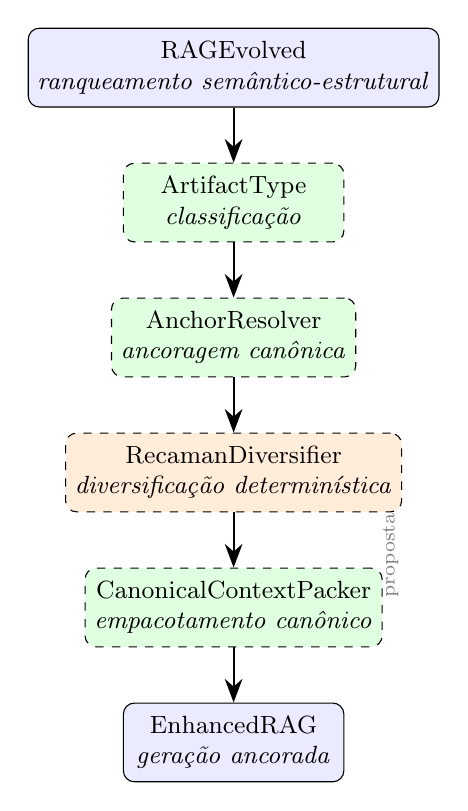
\begin{tikzpicture}[
  node distance=1.1cm,
  box/.style={draw, rounded corners, minimum width=2.8cm, minimum height=1.0cm,
              align=center, font=\small, fill=blue!8},
  prop/.style={draw, rounded corners, minimum width=2.8cm, minimum height=1.0cm,
               align=center, font=\small, fill=green!12, dashed},
  arrow/.style={-{Stealth[length=3mm]}, thick}
]
  \node[box] (ev) {RAGEvolved\\\emph{ranqueamento semântico-estrutural}};
  \node[prop, below=0.7cm of ev] (at) {ArtifactType\\\emph{classificação}};
  \node[prop, below=0.7cm of at] (ar) {AnchorResolver\\\emph{ancoragem canônica}};
  \node[prop, below=0.7cm of ar, fill=orange!15] (rd) {RecamanDiversifier\\\emph{diversificação determinística}};
  \node[prop, below=0.7cm of rd] (cp) {CanonicalContextPacker\\\emph{empacotamento canônico}};
  \node[box, below=0.7cm of cp] (en) {EnhancedRAG\\\emph{geração ancorada}};

  \draw[arrow] (ev) -- (at);
  \draw[arrow] (at) -- (ar);
  \draw[arrow] (ar) -- (rd);
  \draw[arrow] (rd) -- (cp);
  \draw[arrow] (cp) -- (en);

  \node[rotate=90, font=\scriptsize, gray, right=0.1cm of cp] {proposta};
\end{tikzpicture}
\caption{Diagrama da arquitetura-alvo pós-Recamán (proposta). \textbf{Legenda:}
caixas tracejadas verdes = novos artefatos propostos; caixa laranja tracejada =
Diversificador de Recamán (núcleo da proposta); caixas azuis sólidas = componentes
já implementados. Setas = fluxo de dados proposto.}
\label{fig:alvo}
\end{figure}

\subsection*{4.4 Demonstração do Diversificador}

Dada uma sequência ranqueada $\mathbf{r} = [r_1, r_2, \dots, r_N]$ de candidatos e
os termos da sequência de Recamán $a_0, a_1, \dots$, o diversificador proposto
seleciona candidatos percorrendo $\mathbf{r}$ com passos $a_k$, garantindo que
índices próximos (semanticamente redundantes) sejam alternados com saltos
diversificados. A Tabela~\ref{tab:offsets} ilustra os primeiros passos.

\begin{table}[!htb]
\centering
\caption{Passos derivados da sequência de Recamán para diversificação (proposta).
\textbf{Legenda:} $n$ = passo; $a_n$ = valor da sequência; exemplo de índice de
candidato selecionado sobre um ranking fictício.}
\label{tab:offsets}
\begin{tabular}{cccc}
\toprule
$n$ & $a_n$ & índice candidato $(1\!+\!a_n \bmod N)$ & ilustração \\
\midrule
0 & 0 & 1 & primeiro candidato (relevância máxima) \\
1 & 1 & 2 & deslocamento de 1 posição \\
2 & 3 & 4 & salto de 3 posições (diversidade) \\
3 & 6 & 7 & salto maior \\
4 & 2 & 3 & volta a um candidato próximo \\
5 & 7 & 8 & novo salto \\
\bottomrule
\end{tabular}
\end{table}

A Tabela~\ref{tab:offsets} evidencia a alternância entre saltos curtos e longos,
característica da sequência de Recamán, que favorece a cobertura de diferentes
regiões do ranking.

% =====================================================================
\section*{5. Cálculos e Especificações Técnicas}
\addcontentsline{toc}{section}{5. Cálculos e Especificações Técnicas}
% =====================================================================

Esta seção formaliza métricas e especificações associadas à proposta e ao estado
atual.

\subsection*{5.1 Métricas de diversidade}

Sobre um conjunto de candidatos selecionados $\mathcal{S}$, podemos definir a
diversidade média ímpar entre os itens recuperados:

\begin{equation}
\label{eq:diversity}
\text{Div}(\mathcal{S})\;=\;\frac{1}{|\mathcal{S}|(|\mathcal{S}|-1)}
\sum_{i \neq j}\bigl(1 - \text{Sim}(r_i, r_j)\bigr)
\end{equation}

onde $\text{Sim}(\cdot,\cdot) \in [0,1]$ é uma medida de similaridade normalizada
(coseno ou Jaccard sobre âncoras). Valores de $\text{Div}(\mathcal{S})$ próximos
de 1 indicam alta diversidade.

\subsection*{5.2 Custo computacional do Diversificador}

A sequência de Recamán até o passo $M$ pode ser gerada em $O(M)$ com memória
$O(M)$ (mantendo o conjunto dos valores já visitados). Para um corpus de $N$
candidatos e um orçamento de $K$ seleções, o Diversificador proposto opera, no
pior caso, em $O(K)$ sobre o ranking indexado, com memória adicional $O(N)$ para
as âncoras e $O(N)$ para o conjunto de valores da sequência. Isso torna o estágio
assintoticamente barato em relação à codificação dos documentos.

\subsection*{5.3 Antes/depois: contrato da especificação}

A Tabela~\ref{tab:spec} resume as especificações técnicas do estado atual e da
arquitetura-alvo proposta.

\begin{table}[!htb]
\centering
\caption{Especificações técnicas comparadas: estado atual vs.\ proposta
pós-Recamán. \textbf{Legenda:} CH = implementado no checkout; PROP = proposta não
implementada.}
\label{tab:spec}
\begin{tabularx}{\textwidth}{lXX}
\toprule
\textbf{Aspecto} & \textbf{Estado atual} & \textbf{Proposta (pós-Recamán)} \\
\midrule
Ranqueamento primário & BM25/denso (Eq.~\ref{eq:bm25}) & preservado, sem alteração \\
Roteamento adaptativo & \texttt{AdaptiveRetriever} (CH) & preservado \\
Diversificação & via MMR conceitual & \texttt{RecamanDiversifier} (PROP) \\
Classificação de artefato & ausente & \texttt{ArtifactType} (PROP) \\
Ancoragem canônica & parcial (auditoria) & \texttt{AnchorResolver} (PROP) \\
Empacotamento & \texttt{CanonicalContextPacker} (PROP) & proposto \\
Reprodutibilidade da diversif. & não determinística & determinística (Recamán) \\
\bottomrule
\end{tabularx}
\end{table}

% =====================================================================
\section*{6. Implementações Reproduzíveis}
\addcontentsline{toc}{section}{6. Implementações Reproduzíveis}
% =====================================================================

\subsection*{6.1 Geração determinística da sequência de Recamán}

O Algoritmo~\ref{alg:recaman} gera os primeiros $M$ termos da sequência de
Recamán (Eq.~\ref{eq:recaman}). Sua execução é totalmente reprodutível.

\begin{algorithm}[!htb]
\caption{Geração determinística da sequência de Recamán}
\label{alg:recaman}
\begin{algorithmic}[1]
\Require $M \geq 1$ (número de termos desejado), com $a_0 = 0$
\Ensure $a[0..M]$ tais que satisfaçam a Eq.~\ref{eq:recaman}
\State $a[0] \gets 0$
\State $\text{seen} \gets \{0\}$
\For{$n \gets 1$ \textbf{to} $M$}
  \State $\text{cand} \gets a[n-1] - n$
  \If{$\text{cand} > 0$ \textbf{and} $\text{cand} \notin \text{seen}$}
    \State $a[n] \gets \text{cand}$
  \Else
    \State $a[n] \gets a[n-1] + n$
  \EndIf
  \State $\text{seen} \gets \text{seen} \cup \{a[n]\}$
\EndFor
\State \Return $a$
\end{algorithmic}
\end{algorithm}

\subsection*{6.2 Esboço da interface do Diversificador}

O trecho abaixo esquematiza a interface proposta (não implementada) do
\texttt{RecamanDiversifier}:

\begin{lstlisting}[language=Python, caption={Esboço de interface do RecamanDiversifier (proposta, não implementada).}]
class RecamanDiversifier:
    """Deterministic diversifier based on the Recaman sequence.

    PROPOSAL - NOT implemented in the checkout.
    """
    def __init__(self, seen=None):
        self.a = [0]
        self.seen = seen or {0}

    def next_offset(self, n):
        # generates a_n per the Recaman Eq. (O(1) amortized)
        prev = self.a[n - 1]
        cand = prev - n
        if cand > 0 and cand not in self.seen:
            val = cand
        else:
            val = prev + n
        self.a.append(val)
        self.seen.add(val)
        return val

    def diversify(self, ranked, k):
        """Selects k candidates from 'ranked' using Recaman offsets."""
        selected = []
        cursor = 0
        n = 0
        while len(selected) < k and cursor < len(ranked):
            selected.append(ranked[cursor])
            offset = self.next_offset(n)
            cursor = (cursor + offset + 1) % len(ranked)
            n += 1
        return selected
\end{lstlisting}

\subsection*{6.3 Compilação do manual}

O PDF deste manual é compilado de forma reproduzível com os comandos:

\begin{lstlisting}[language=bash, caption={Comando de compilação reproduzível do manual.}]
cd docs/r456_manual_tecnico_rag
./build.sh            # uses pdflatex + bibtex + makeindex
# or, alternatively:
make                  # uses latexmk -pdf
\end{lstlisting}

A toolchain exigida é TeX Live com \texttt{pdflatex}, \texttt{bibtex},
\texttt{makeindex} e \texttt{latexmk}, e a classe local
\texttt{abntex2} do diretório \texttt{publishing/templates/abntex2}.

% =====================================================================
\section*{7. Mapas de Dados e Diagrama Operacional}
\addcontentsline{toc}{section}{7. Mapas de Dados e Diagrama Operacional}
% =====================================================================

O ecossistema mantém mapas de dados e mapas de arquitetura em
\texttt{docs/} (por exemplo, \texttt{MAPA\_ARQUITETURA\_R433\_R438.md},
\texttt{architecture\_map.html}). Estes artefatos documentais informam tanto o
estado atual quanto o desenho da proposta, preservando a riqueza dos fluxos
multiárea (acadêmico, formal, jurídico, clínico, MIRA, RAG, Universidade
Sintética, runtimes locais e gates de qualidade/integridade).

\subsection*{7.1 Integração do RAG nos fluxos multiárea}

O RAG atua como subsistema transversal: serve ao fluxo acadêmico (revisão de
literatura), ao fluxo jurídico (recuperação normativa), ao fluxo clínico
(suporte à decisão) e ao fluxo MIRA (geração de conteúdo). A proposta de
diversificação por Recamán visa melhorar a cobertura semântica desse subsistema
transversal, sem alterar a interface pública dos fluxos consumidores.

% =====================================================================
\section*{8. Considerações Finais e Trabalho Futuro}
\addcontentsline{toc}{section}{8. Considerações Finais e Trabalho Futuro}
% =====================================================================

Este manual documentou o estado atual da arquitetura RAG e apresentou, de forma
rigorosamente rotulada, uma proposta de diversificação estruturada baseada na
sequência de Recamán. Os pontos centrais são:

\begin{enumerate}[label=\arabic*.]
  \item O estado atual é observável em \texttt{rag/evolved.py} e
        \texttt{rag/enhanced\_search\_rag.py}, cobrindo ranqueamento adaptativo,
        busca unificada, síntese e auditoria bibliográfica.
  \item A arquitetura-alvo pós-Recamán é \textbf{proposta}, introduzindo
        \texttt{ArtifactType}, \texttt{AnchorResolver},
        \texttt{RecamanDiversifier} e \texttt{CanonicalContextPacker}.
  \item A diversificação é determinística e de baixo custo assimptótico,
        alinhada ao espírito de MMR e apoiada em referências reais.
\end{enumerate}

Como \textbf{trabalho futuro}, recomenda-se: (i) implementar o
\texttt{RecamanDiversifier} seguindo o protocolo TDD; (ii) medir a métrica de
diversidade (Eq.~\ref{eq:diversity}) em um corpus-piloto; (iii) comparar o
desempenho com MMR e com o estado atual; e (iv) registrar cada ciclo de evolução
no \texttt{evolution/cycles.json} e no MetaBus, conforme o protocolo do
ecossistema.

% =====================================================================
% Referências
% =====================================================================
\clearpage
\bibliography{referencias}
\bibliographystyle{abntex2-alf}

\end{document}
